\scanpage{67}\mspage{66}
% The raised inclusion and the long connecting stroke below the second row
% are reproduced with their formula labels; the labels occur only here.
\figure{%
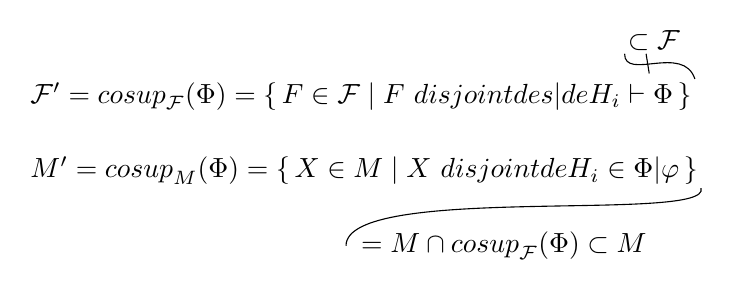
\begin{tikzpicture}[every node/.style={inner sep=1pt}]
\node[anchor=west] (topone) at (0,0) {$\mathcal F'=\operatorname{cosup}_{\mathcal F}(\Phi)=\{\,F\in\mathcal F\mid F\ \text{disjoint \unsure{des|de} }H_i\vdash\Phi\,\}$};
\node[anchor=south east] (inc) at ([xshift=-.15cm,yshift=.32cm]topone.north east) {$\inserted{\subset\mathcal F}$};
\draw (inc.south west) .. controls +(0,-.35) and +(-.15,.45) .. (topone.north east);
\draw ([xshift=-.47cm]inc.south east) -- ++(.04,-.25);
\node[anchor=west] (toptwo) at (0,-.95) {$M'=\operatorname{cosup}_{M}(\Phi)=\{\,X\in M\mid X\ \text{disjoint de }H_i\in\unsure{\Phi|\varphi}\,\}$};
\node[anchor=west] (topthree) at (4.2,-1.9) {$\inserted{=M\cap\operatorname{cosup}_{\mathcal F}(\Phi)\subset M}$};
\draw (toptwo.south east) .. controls +(.15,-.45) and +(0,.8) .. ([xshift=-.15cm]topthree.west);
\end{tikzpicture}%
}

\deleted{Donc \unsure{on aura|on a}, pour $F\in\mathcal F$ posant $\mathcal F'=\operatorname{cosup}_{\mathcal F}$,}

\[
\begin{aligned}
&\deleted{\unsure{\phi|\Phi}}\qquad
\deleted{\mathcal F'=\operatorname{cosupp}_{\mathcal F}(\Phi),\quad M'=\mathcal F'\cap M,}\\[-2pt]
&\qquad\deleted{F\in\operatorname{cosup}_{\unsure{,|\mathcal F}}}
\qquad\qquad\deleted{=\operatorname{cosup}_{\deleted{\unsure{\mathcal F}}M}(\mathcal F)}
\end{aligned}
\]

Donc pour $F\in\mathcal F$

% Slanted left marginal note, the brace display, and the right marginal
% note are one graphical group. Neither margin text is duplicated.
\figure{%
\begin{tikzpicture}[every node/.style={inner sep=1pt}]
\node[anchor=west,rotate=13,align=left] (leftnote) at (0,-.5)
 {Ainsi, $M'$ et $\mathcal F'$\\se déterminent\\\unsure{mutuellement}};
\node[anchor=west] (braced) at (3.5,0)
 {$\left\{\begin{aligned}
 F\in\mathcal F'&\Longleftrightarrow\overline F\subset M'\\
 M'&=.\mathcal F'\cap M
 \end{aligned}\right.$};
\draw[->] ([xshift=-.8cm,yshift=.12cm]braced.west) -- ([xshift=-.35cm,yshift=.2cm]braced.west);
\node[anchor=north west,align=left] (nb) at (11.2,.75)
 {NB $\mathcal F',M'$\\sont des\\parties\\fermées de\\$\mathcal F,M$.};
\node[anchor=west] (subject) at (9.9,-1.55) {$\mathcal F'$};
\node[anchor=west] (stable) at (9.9,-2.1) {\uline{Stable par Sup.}};
\draw ([xshift=-.05cm,yshift=-.04cm]subject.south west) -- ([xshift=.25cm,yshift=-.04cm]subject.south east) -- ++(0,.35);
\draw ([xshift=-1.5cm,yshift=.15cm]stable.west)
 .. controls +(1,.15) and +(-.6,.4) .. ([xshift=-.2cm]stable.west)
 .. controls +(-.2,-.4) and +(-.7,0) .. ([xshift=.2cm,yshift=-.2cm]stable.south east);
\draw ([xshift=-.05cm]subject.south west)
 .. controls +(-.5,-.2) and +(-.5,0) .. ([xshift=-.1cm,yshift=-.18cm]stable.south west)
 -- ([xshift=.1cm,yshift=-.18cm]stable.south east)
 -- ++(.5,-.4);
\end{tikzpicture}%
}

Soit d'autre part
\[
\begin{aligned}
\mathcal F''&=\operatorname{cosupp}_{\mathcal F}(\mathcal F')\overset{\text{def}}{=}\operatorname{supp}_{\mathcal F}(\Phi)\\
M''&=\operatorname{cosup}_{M}(\mathcal F')\overset{\text{def}}{=}\operatorname{supp}_{M}(\Phi)
\end{aligned}
\]

On a \unsure{vu|bien|la|là} $\mathcal F''\supset\Phi$, $\mathcal F''$ stable par \unsure{Sup|Supp}, \deleted{contient $\Phi$} et par passage \unsure{:|à} une sous-figure. Soit $\deleted{\unsure{M}}\overline\Phi=\bigcup_{H_i\in\Phi}\overline H_i$, alors
\[
\begin{aligned}
\operatorname{cosup}_{\mathcal F}(\Phi)&=\operatorname{cosup}_{\mathcal F}(M_{\overline\Phi})\\
\operatorname{cosup}_{\deleted{\unsure{\mathcal F}}M\unsure{..|:}}(\Phi)&=\{\,\deleted{\unsure{\varnothing|x}}X\in M\mid X\ \text{disjoint de }\unsure{\mathrm{tt}|\forall}\ Y\in M_{\overline\Phi}\,\}
\end{aligned}
\]
donc on est \unsure{ramené|revenu} à des constructions dans $M$. \S

\uline{Partie saturée \inserted{$\mathcal F_0$} de} $\deleted{\unsure{M}}\mathcal F$ : égale au cosupport de son cosupport ($\text{p. r. à }\mathcal F$). Partie \unsure{saturée|saturee} \inserted{$M_0$} de $M$ : égale au cosupport de son support (dans $M$). Elles se correspondent \unsure{mutuellement} \unsure{par|\deleted{par}}
\[
\begin{aligned}
M_0&=\mathcal F_0\cap M\\
\mathcal F_0&=\{\,F\in\mathcal F\mid\overline F\subset M_0\,\}
\end{aligned}
\]
